%%%%%%%%%%%%%%%%%%%%%%%%%%%%%%%%%%%%%%%%%
% University Assignment Title Page 
% LaTeX Template
% Version 1.0 (27/12/12)
%
% This template has been downloaded from:
% http://www.LaTeXTemplates.com
%
% Original author:
% WikiBooks (http://en.wikibooks.org/wiki/LaTeX/Title_Creation)
%
% License:
% CC BY-NC-SA 3.0 (http://creativecommons.org/licenses/by-nc-sa/3.0/)
%
%%%%%%%%%%%%%%%%%%%%%%%%%%%%%%%%%%%%%%%%%
%\title{Title page with logo}
%----------------------------------------------------------------------------------------
%	PACKAGES AND OTHER DOCUMENT CONFIGURATIONS
%----------------------------------------------------------------------------------------

\documentclass[12pt]{article}
\usepackage[english]{babel}
\usepackage[utf8x]{inputenc}
\usepackage{natbib}
\usepackage{color}
\usepackage[explicit]{titlesec}
\usepackage{url}
\usepackage{graphicx}
\usepackage[section]{placeins}
\usepackage{chngcntr}
\usepackage{subcaption}

\counterwithin*{section}{part}


\begin{document}

\begin{titlepage}

\newcommand{\HRule}{\rule{\linewidth}{0.5mm}} % Defines a new command for the horizontal lines, change thickness here

\center % Center everything on the page
 
%----------------------------------------------------------------------------------------
%	HEADING SECTIONS
%----------------------------------------------------------------------------------------

\textsc{\LARGE University of St Andrews}\\[1.5cm] % Name of your university/college
\textsc{\Large CS5014 }\\[0.5cm] % Major heading such as course name
\textsc{\large Practical 1}\\[0.5cm] % Minor heading such as course title

%----------------------------------------------------------------------------------------
%	TITLE SECTION
%----------------------------------------------------------------------------------------

\HRule \\[0.4cm]
{ \huge \bfseries Machine Learning}\\[0.4cm] % Title of your document
\HRule \\[1.5cm]
 
%----------------------------------------------------------------------------------------
%	AUTHOR SECTION
%----------------------------------------------------------------------------------------


\Large \emph{Author:}\\
 \textsc{150008022}\\[3cm] % Your name

%----------------------------------------------------------------------------------------
%	DATE SECTION
%----------------------------------------------------------------------------------------

{\large \today}\\[2cm] % Date, change the \today to a set date if you want to be precise

%----------------------------------------------------------------------------------------
%	LOGO SECTION
%---------------------------------------------------------------------------------------


\includegraphics[width = 3.1cm]{images/standrewslogo.png}
 
%----------------------------------------------------------------------------------------

\vfill % Fill the rest of the page with whitespace

\end{titlepage}

\pagenumbering{gobble}

\part*{Goal}

The goal of this practical was to cleanse and process real world data in order to produce a regression model, and evaluate its performance.

\tableofcontents

\pagebreak

\pagenumbering{arabic}
\setcounter{page}{1}

\part{Loading and Cleaning the Data}

\section{Loading}
Numpy was used to load the csv file. The header row was skipped, and to ensure there were no missing values, the invalid raise flag was also used when parsing the data. This would raise an exception if any rows were found to be missing data. 

No preproccessing had occurred on the data set according to the original paper, and so the data could be used as given.

The input and output columns were separated into two variables x and y, in accordance with the notation used in lectures.

\section{Data Splitting}

Next, the testing set was isolated from the available data. Simple random sampling (SRS) and stratified sampling were considered for performing the data splitting. SRS is intuitive, but for less uniformly distributed data sets, it can lead to subsets that poorly represent the input data, and therefore suffer from sampling bias \cite{reitermanova_2010}. 

For these reasons, stratified random sampling was used with a 80\%-20\% split.  To ensure our training and testing sets were representative of our data, the output variables were used to categorise the data into strata. Since the two appeared to have a linear relationship as shown in figure \ref{fig:y1vsy2}, we could assume that using one column for categorising our data would produce an roughly equal distribution of the values in both columns.

The 586 possible values of Y1 were split into 50 bins using \url{numpy.digitize}, and then passed to \url{train_test_split} as the \url{stratify} argument. 

\part{Analysing and Visualising the Data}

\section{Distributions}

Firstly, a histogram of each of the input variables and outputs were plotted in order to visualise the distribution of the values (Figures \ref{fig:xdist} and \ref{fig:ydist}). When comparing to the histograms from the given paper \cite{tsanas_xifara_2012}, most of the plots matched. Any differences were identified to be caused by 10 bins always being used (the default if not specified by numpy.hist), and the paper would sometimes use more. However, it was still clear that none of the variables had a gaussian distribution. The output variables also appeared tail heavy, but the inputs did not.

\begin{figure}[!ht]
\centering
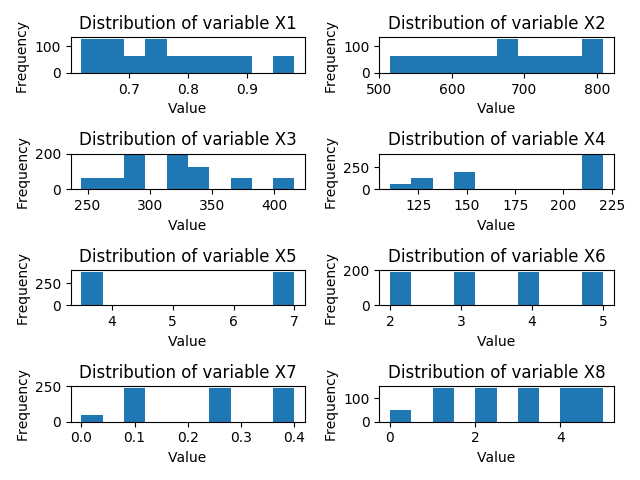
\includegraphics[width=0.8 \linewidth]{images/XDist}
\caption{Distribution of input variables}
\label{fig:xdist}
\end{figure}

\begin{figure}[!ht]
\centering
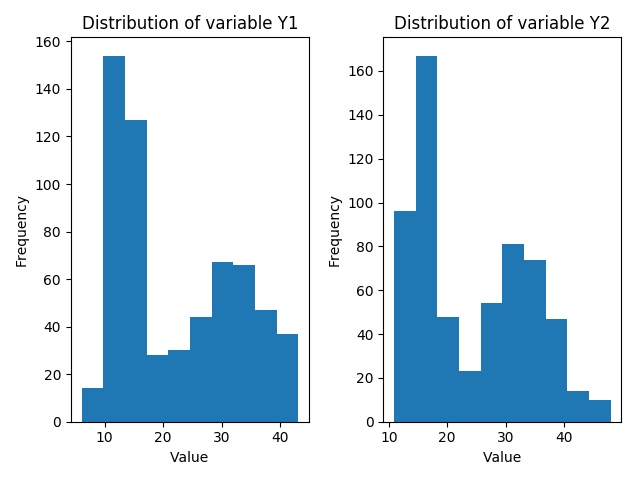
\includegraphics[width=0.8 \linewidth]{images/YDist}
\caption{Distribution of output variables}
\label{fig:ydist}
\end{figure}

\FloatBarrier

\section{Relationships}

In order to identify which variables had the strongest relationships with the outputs, and if these relationships were linear or monotonic, scatter graphs were made between each input and output variable (Figures \ref{fig:xvsy0} and \ref{fig:xvsy1}). The inputs were normalised to allow for comparisons between values that could have very different ranges. To better visualise the density of the data points as well as their position, the \url{alpha} parameter was set to 0.1 in the plots. 

\begin{figure}[!ht]
\centering
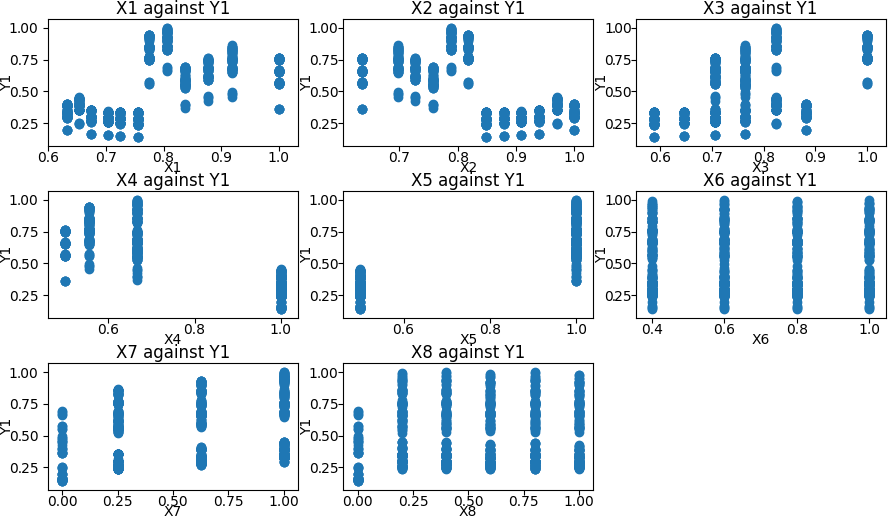
\includegraphics[width=0.8 \linewidth]{images/XsVsY0}
\caption{Normalised inputs plotted against the first output variable}
\label{fig:xvsy0}
\end{figure}

\begin{figure}[!ht]
\centering
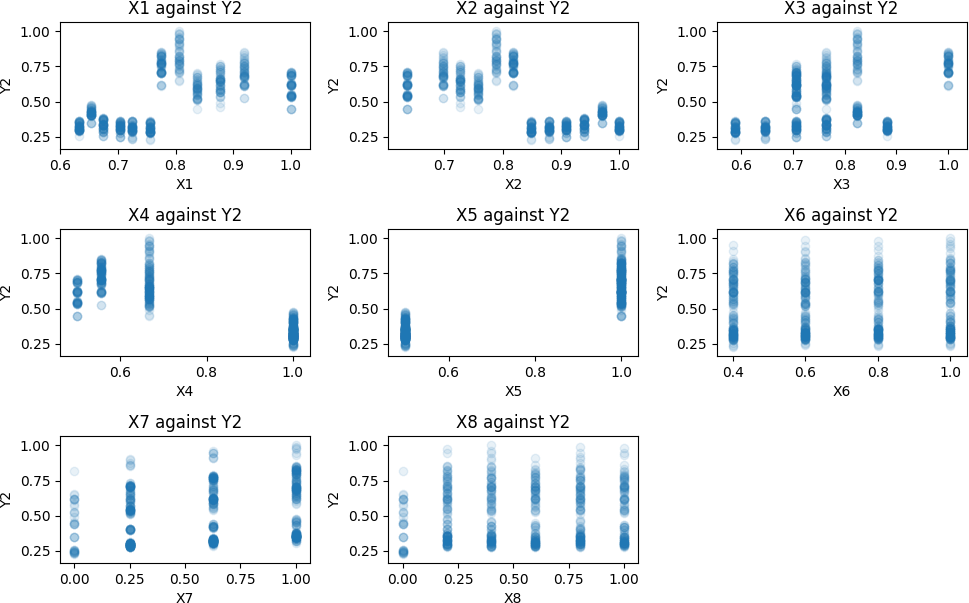
\includegraphics[width=0.8 \linewidth]{images/XsVsY1}
\caption{Normalised inputs plotted against the second output variable}
\label{fig:xvsy1}
\end{figure}

\FloatBarrier

Since the distribution of the outputs were so similiar, they were also plotted against each other in a scatter plot (Figure \ref{fig:y1vsy2}). This showed that the two variables had very similiar values, and so a regression model that applied to only one of them could likely be used for the other.

\begin{figure}[!ht]
\centering
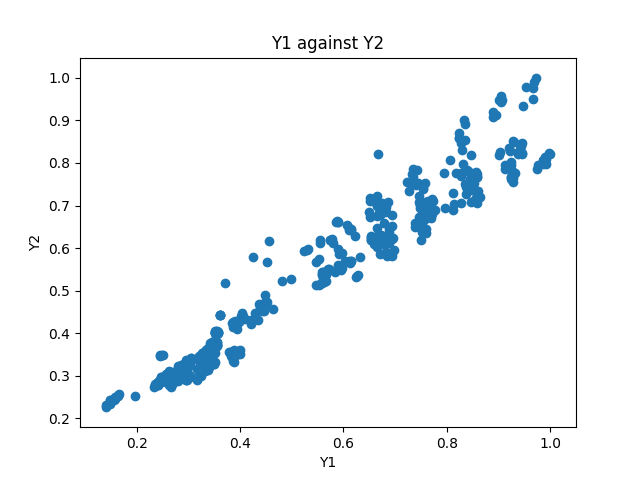
\includegraphics[width=0.8 \linewidth]{images/Y1vsY2}
\caption{Normalised outputs against each other}
\label{fig:y1vsy2}
\end{figure}

\FloatBarrier

\part{Feature Selection}

\section{Correlation Ranking}

To try and identify which features had the strongest effect on the outputs, both the Pearson and Spearman rank correlation coefficients were considered. It was noted that the Pearson correlation would give a perfect value when the two variables were linearly related, whilst the Spearman correlation (a similiar alternative, and the one used in the original paper) would give a perfect value when the variables were monotonically related. Given these factors, the Spearman rank correlation coefficient was used as a filter method.

From the scatter plots, some variables appeared to have a possible linear relationship with the outputs (for example, X7 and Y1), whilst others had a monotonic relationship (for example, X1 and Y1). Using the Scipy \emph{stats.spearmanr} method, the correlation coefficients were easily calculated, alongside a p-value, as shown in table \ref{tbl:spearman-table}. Immediately from these result we can see that X6 and X8 show little evidence of a monotonic relationship existing between them and either of the outputs. 

However, according to Schiavon et al. \cite{schiavon_lee_bauman_webster_2010}, the orientation (X6) is one of the most important predictors for cooling load (Y2). Though fewer features would improve the processing time, and removing less important features would be crucial for  eliminating noise, only X8 was removed from our feature set.

\begin{table}[!ht]
\centering
\begin{tabular}{||l|l|l|l||}
\hline
X    				& Y & Rho   & p    \\
\hline
1                   & 1 & 0.61  & 0.00 \\
1                   & 2 & 0.64  & 0.00 \\
2                   & 1 & -0.61 & 0.00 \\
2                   & 2 & -0.64 & 0.00 \\
3                   & 1 & 0.49  & 0.00 \\
3                   & 2 & 0.43  & 0.00 \\
4                   & 1 & -0.80 & 0.00 \\
4                   & 2 & -0.80 & 0.00 \\
5                   & 1 & 0.86  & 0.00 \\
5                   & 2 & 0.86  & 0.00 \\
6                   & 1 & 0.00  & 0.99 \\%
6                   & 2 & 0.03  & 0.51 \\
7                   & 1 & 0.35  & 0.00 \\
7                   & 2 & 0.32  & 0.00 \\
8                   & 1 & 0.09  & 0.03 \\
8                   & 2 & 0.06  & 0.14 \\
\hline
\end{tabular}
\caption{Spearman rank correlation coefficients, with p values}
\label{tbl:spearman-table}
\end{table}

\part{Selecting and Training a Regression Model}

\section{Model Selection}
The limited size of the corpus available made the choice of algorithm especially crucial. The lack of noticable outliers in the visualistions at least suggest that the data is not of poor-quality. 

Scikit-Learns \url{DecisionTreeRegressor} \cite{scikitlearntree} which implements CART was used as the regression model due to the complex relationships that appeared to exist between the inputs and outputs, using mean squared error as the cost function.

Linear regression was deemed inappropriate as it is a global model. The relationships between the inputs as well as their individual valuddces seemed to have an effect on the output, and so a model that captured these inter-variable relationships would likely be more effective. The danger with using CART was that it could be more prone to overfitting, but placing limits on the complexity of the decision tree could reduce this risk. 

\begin{figure}[!ht]
\centering
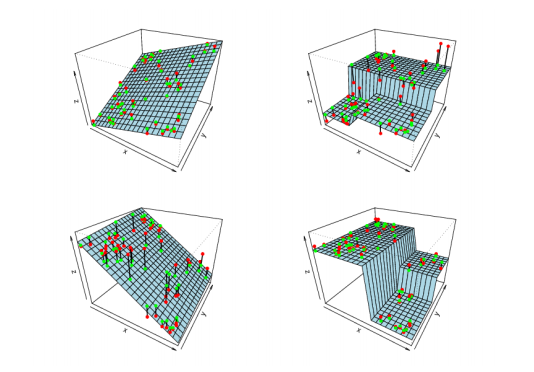
\includegraphics[width=0.8 \linewidth]{images/cartvslinear}
\caption{Comparison of CART and Linear Regression \cite{breiman}}
\label{fig:cartvslinear}
\end{figure}

The model is constructed by recursively breaking down the training data and building a decision tree from each subsection of the data. The tree can then be used to make a prediction based on some input x by starting at the root node of the tree and using a series of questions to find the leaf node that would be our prediction. For example, one of the questions might be "is X1 greater than 0.5?" or "is X1 greater than X2?". CART constructs a binary decision tree by using the attribute that provides the most information gain at each stage.

\section{Cost Function Selection}

Root Mean Square Error (RMSE) and Mean Absolute Error (MAE) were both considered as performance measures for regression. RMSE minimizes for the squared difference between the estimated and expected values, whilst MAE minimizes for the absolute difference, therefore RMSE is more affected by outliers, which can result in overfitting. However the input data did not seem to contain many outliers, and so RMSE was chosen.

\section{Validation Method}

Due to the relatively small corpus size, K-fold cross-validation was chosen to estimate the model error \cite{gron_2018}. 10 folds were used as it provides a good compromise between bias and variance \cite{hastie01statisticallearning}.

\section{Optimisations}

By assessing the accuracy of the CART model at limited depths, we could attempt to limit the complexity of the decision tree created, and therefore reduce the chance of overfitting. By iteratively using k-fold cross validation and RMSE to produce an accuracy score at increasing depths, we would be able to find the point where increasing complexity does not benefit the model \cite{massaron_mueller_2015}. 

Figure \ref{fig:depth} shows that performance begins to deteriorate once depth is greater than 6. Accuracy alone is not enough to confirm a models effeccd tiveness, but can build confidence in the model when coupled with another method such as cross-validation.

\begin{figure}[!ht]
\centering
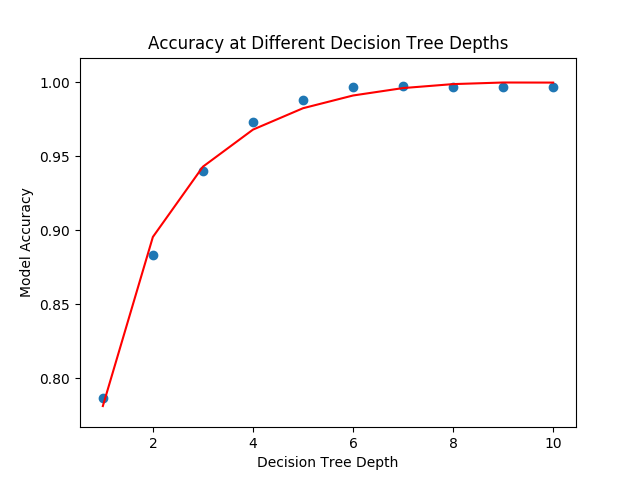
\includegraphics[width=0.8 \linewidth]{images/depth}
\caption{Accuracy of model with increasing decision tree depth}
\label{fig:depth}
\end{figure}

\section{Other Observations}

Out of curiosity, the 'importance' of each variable was also plotted to better understand what the regression model would be most affected by, and to see if this aligned with the feature selection methods used earlier.

Figure \ref{fig:fi} shows that the two models are strongly dependent on different variables. Relative compactness has the strongest effect on the heating load, whilst overall height has the strongest effect on the cooling load.

This is not the expected result based on the spearman rank correlation coefficients calculated in table \ref{tbl:spearman-table}. There also appears to be very little dependence in both models on X6 despite the results referred to from Schiavon et al \cite{schiavon_lee_bauman_webster_2010}.

When the \url{

\begin{figure}[!ht]
\centering
\begin{subfigure}{.5\textwidth}
  \centering
  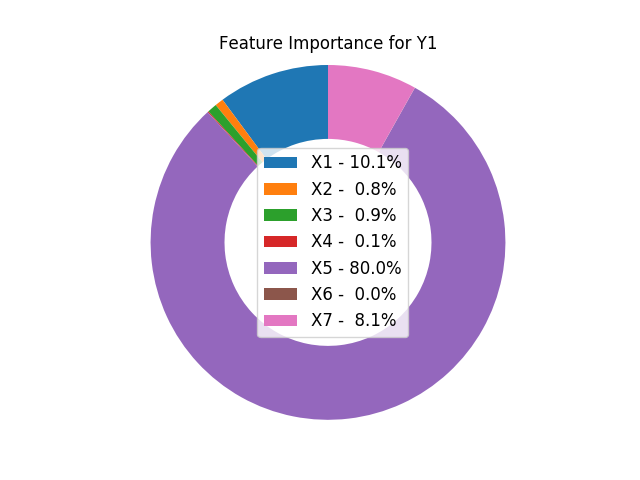
\includegraphics[width=\linewidth]{images/fiY1}
  \caption{Feature Importance for Y1}
  \label{fig:fiy1}
\end{subfigure}%
\begin{subfigure}{.5\textwidth}
  \centering
  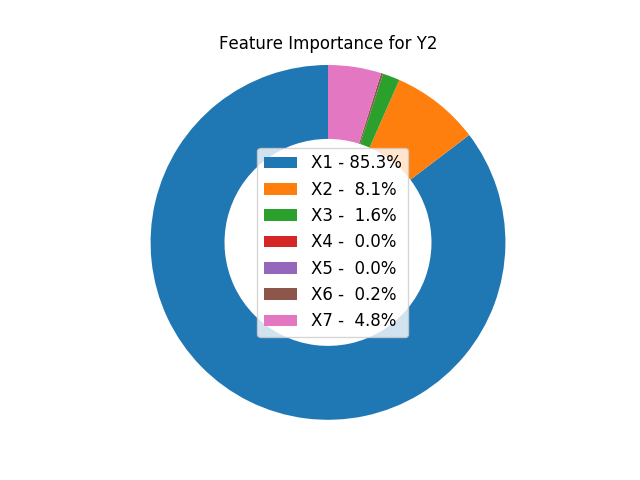
\includegraphics[width=\linewidth]{images/fiY2}
  \caption{Feature Importance for Y2}
  \label{fig:fiy2}
\end{subfigure}
\caption{Feature Importance for models trained on the different outputs}
\label{fig:fi}
\end{figure}

\FloatBarrier

\part{Performance Evaluation}

\section{Results}

The model was trained on the training data with the max depth set to 6, and then used to predict the outputs using the test data isolated earlier. A seperate model was used for predicting each of the output variables. The differences between the predicted values and actual values are visualised in figures \ref{fig:y1error} and \ref{fig:y2error}.

\begin{figure}[!ht]
\centering
\begin{subfigure}{.5\textwidth}
  \centering
  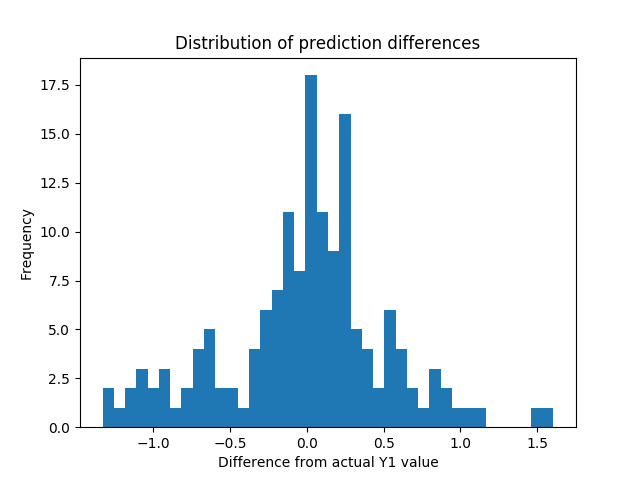
\includegraphics[width=\linewidth]{images/Y1errordist}
  \caption{Distribution of differences for Y1}
  \label{fig:y1diffdist}
\end{subfigure}%
\begin{subfigure}{.5\textwidth}
  \centering
  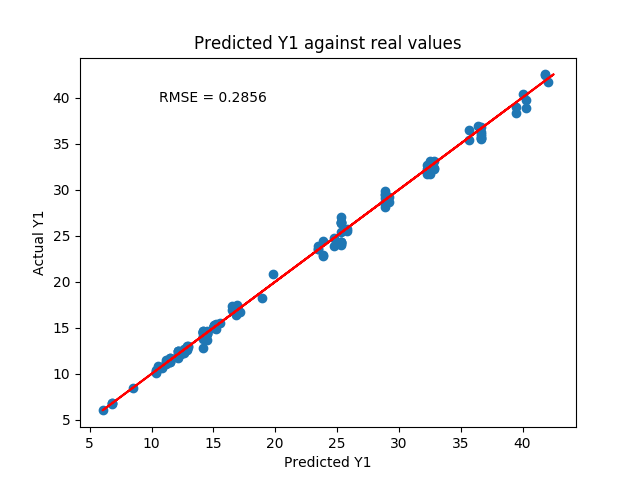
\includegraphics[width=\linewidth]{images/Y1scatter}
  \caption{Prediction against Actual for Y1}
  \label{fig:y1diffscatter}
\end{subfigure}
\caption{Error visualisation for Y1}
\label{fig:y1error}
\end{figure}

\begin{figure}[!ht]
\centering
\begin{subfigure}{.5\textwidth}
  \centering
  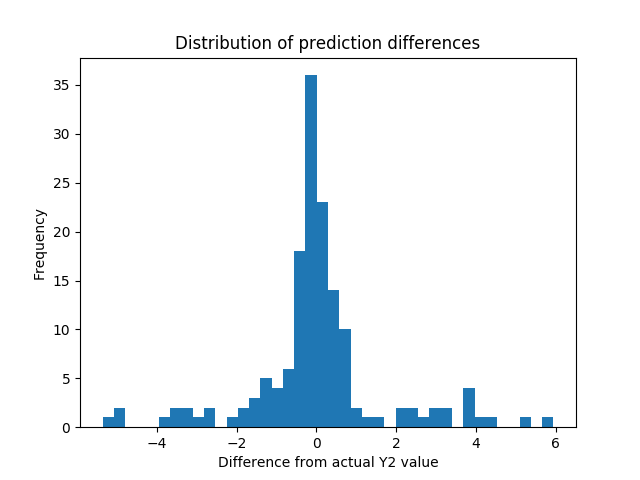
\includegraphics[width=\linewidth]{images/Y2errordist}
  \caption{Distribution of differences for Y2}
  \label{fig:y2diffdist}
\end{subfigure}%
\begin{subfigure}{.5\textwidth}
  \centering
  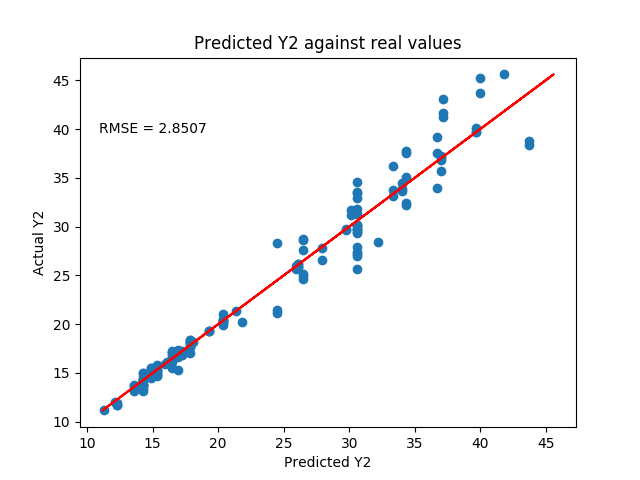
\includegraphics[width=\linewidth]{images/Y2scatter}
  \caption{Prediction against Actual for Y2}
  \label{fig:y2diffscatter}
\end{subfigure}
\caption{Error visualisation for Y}
\label{fig:y2error}
\end{figure}

\section{Evaluation}

The model seems to perform well with both outputs, and especially with Y1, based solely on the RMSE values. \#TODO

\part{Discussion}

\#TODO

\part{Conclusion}

\#TODO

\bibliographystyle{unsrt}
\bibliography{mybib}

\end{document}
